\chapter*{附录：曲线及其亏格}

\section{非奇异三次曲线的拓扑}

我们不难看出，一条非奇异的实平面三次曲线 \(C: y^2 = x^3 + ax + b \subset \mathbb{P}^2_\mathbb{R}\) 具有以下两种形态之一：

\begin{figure}[ht]
\centering
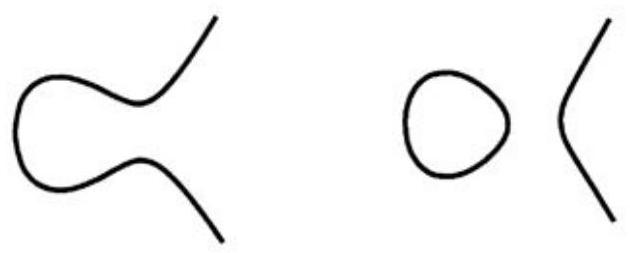
\includegraphics[max width=0.4\textwidth]{images/bo_d3lj80c601uc738kffi0_46_521_964_630_253_0.jpg}
\caption{实三次曲线的两种形态}
\end{figure}

从拓扑角度看，\(C\) 的实部要么是一个圆，要么是两个圆（包含无穷远点）。

为了在复数域 \(\mathbb{C}\) 上考察同样的问题，我们采用另一种标准形式：
\[
C: y^2 = x(x-1)(x-\lambda) \cup \{\infty\}
\]
那么，\(C \subset \mathbb{P}^2_\mathbb{C}\) 的拓扑结构是什么？答案是：一个环面。

\begin{figure}[ht]
\centering
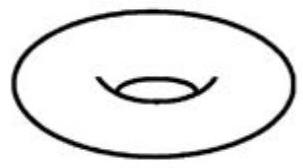
\includegraphics[max width=0.2\textwidth]{images/bo_d3lj80c601uc738kffi0_46_689_1557_303_168_0.jpg}
\caption{环面}
\end{figure}

证明的思路是考虑映射
\[
\pi: C \to \mathbb{P}^1_\mathbb{C} \quad \text{by} \quad (X:Y:Z) \mapsto (X:Z) \quad \text{and} \quad \infty \mapsto (1:0);
\]
在仿射坐标中，这是 \((x,y) \mapsto x\)。因此，这是一个 2-1 映射，对应于 \(y = \pm \sqrt{x(x-1)(x-\lambda)}\) 的图像。我们知道，\(\mathbb{P}^1_\mathbb{C}\) 与黎曼球面同胚（通过球极投影）。现在，我们来考虑定义在 \(\mathbb{P}^1_\mathbb{C}\) 上的“函数” \(y(x) = \pm \sqrt{x(x-1)(x-\lambda)}\)。在分支点 \(\{0, 1, \lambda, \infty\}\) 之外，这是一个二值函数。

\begin{figure}[ht]
\centering
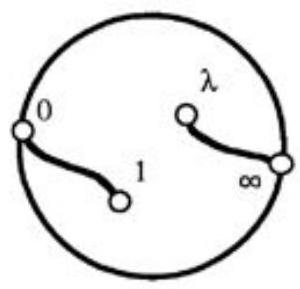
\includegraphics[max width=0.2\textwidth]{images/bo_d3lj80c601uc738kffi0_47_801_471_300_289_0.jpg}
\caption{连接分支点的两条路径：[0,1] 和 [\(\lambda, \infty\)]}
\end{figure}

现在，我们沿着连接分支点的两条路径 [0,1] 和 \([\lambda, \infty]\) 切开黎曼球面 \(\mathbb{P}^1_\mathbb{C}\)。这个二重覆盖分解为两个部分，函数 \(y\) 在每个分支上都是单值的。（阴影表示两张分支的匹配方式）

\begin{figure}[ht]
\centering
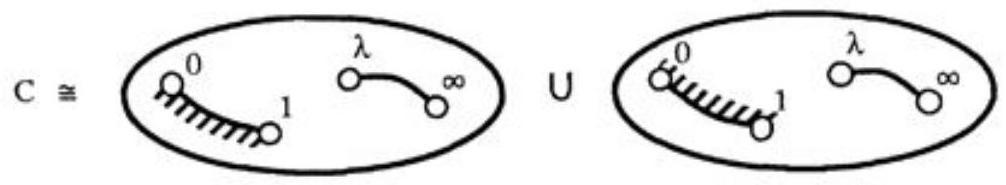
\includegraphics[max width=0.7\textwidth]{images/bo_d3lj80c601uc738kffi0_47_445_997_1006_185_0.jpg}
\caption{\(C\) 作为两个带裂缝球面的并集}
\end{figure}

为了理解其拓扑结构，我们将裂缝打开：

\begin{figure}[ht]
\centering
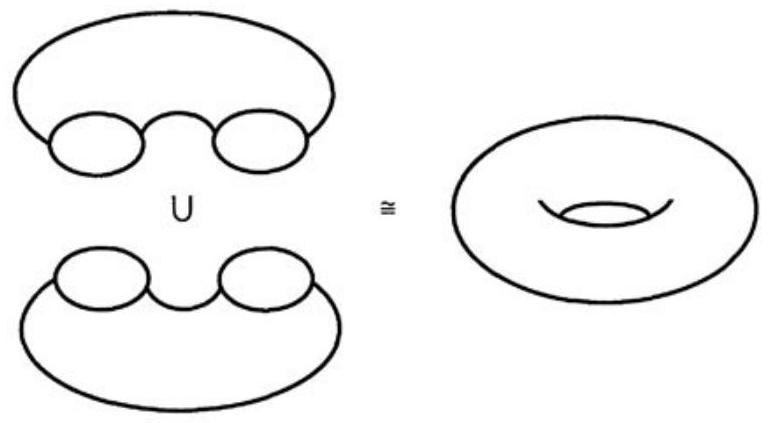
\includegraphics[max width=0.6\textwidth]{images/bo_d3lj80c601uc738kffi0_47_566_1379_768_423_0.jpg}
\caption{将两个带裂缝的球面粘合得到环面}
\end{figure}

\section{关于曲面亏格的讨论}

定义在 \(\mathbb{C}\) 上的非奇异射影曲线 \(C\) 只有一个拓扑不变量，即其亏格 \(g = g(C)\)：

\begin{figure}[ht]
\centering
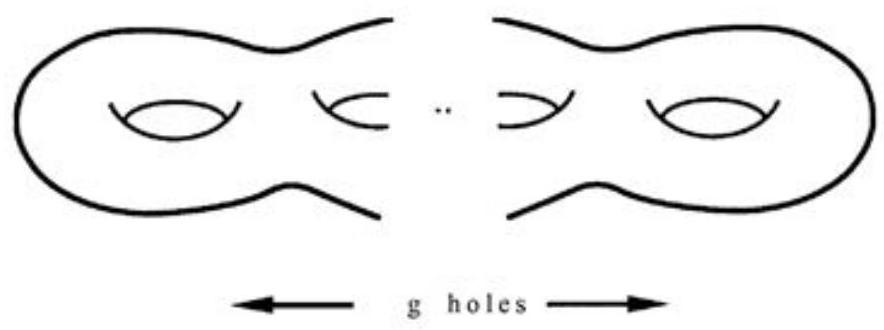
\includegraphics[max width=0.6\textwidth]{images/bo_d3lj80c601uc738kffi0_48_396_449_884_330_0.jpg}
\caption{亏格为 \(g\) 的曲面}
\end{figure}

例如，仿射曲线 \(C: y^2 = f_{2g+1}(x) = \prod_i (x-a_i) \subset \mathbb{C}^2\)，其中 \(f_{2g+1}\) 是一个具有 \(2g+1\) 个不同根 \(a_i\) 的多项式。我们可以像 (2.13) 中那样，将其与 \(\sqrt{f}\) 的黎曼曲面联系起来，并视其为在 \(2g+1\) 个点 \(a_i\) 及无穷远点 \(\infty\) 处分歧的黎曼球面 \(\mathbb{P}^1_\mathbb{C}\) 的二重覆盖。通过相同的论证，可以看出其亏格为 \(g\)。

另一个重要的例子是，一条次数为 \(d\) 的非奇异平面曲线 \(C_d \subset \mathbb{P}^2_\mathbb{C}\) 的亏格由其次数决定，公式为 \(g(C_d) = \binom{d-1}{2}\)。

\section{延伸阅读}

复曲线（即紧致黎曼曲面）出现在数学的各个领域，从丢番图算术、复分析、低维拓扑到数学物理中的微分方程。因此，深入学习复曲线是很有价值的。

曲线的性质在很大程度上由其亏格决定，特别是根据三分法 \(g=0, g=1\) 或 \(g \geq 2\) 来划分。下页的表格描述了其中一些更显著的方面，我们也将进行简要讨论。这些内容应当成为每位数学家的背景知识。

为了部分回答 (1.1-2) 和 (2.1) 中提到的丢番图问题，我们已知一条曲线当且仅当其亏格 \(g=0\) 时，才可以用有理函数参数化。如果我们在一个固定域 \(k\) 上工作，亏格为 0 的曲线可能没有任何 \(k\)-值点（例如 (1.2) 中的圆锥曲线），但如果它有一个 \(k\)-值点，那么它就可以在 \(k\) 上被参数化，使得其 \(k\)-值点与 \(\mathbb{P}^1_k\) 一一对应。

任何亏格为 1 的曲线都同构于本节中的三次曲线，并且在其 \(k\)-值点集上可以定义一个群运算（当然前提是至少存在一个点——不存在空群）。如果 \(k\) 是一个数域（例如 \(k = \mathbb{Q}\)），则其 \(k\)-值点构成一个有限生成的阿贝尔群（莫德尔-韦尔定理）。

对于亏格 \(g \geq 2\) 的曲线，现在已知它们在数域 \(k\) 上只有有限个 \(k\)-值点。这是法尔廷斯（Gerd Faltings）于 1983 年证明的著名定理（该成果为他赢得了 1986 年的菲尔兹奖）。例如，对于任意 \(n \geq 4\)，费马曲线 \(x^n + y^n = 1\) 在有理数上最多只有有限个解。

在 \(\mathbb{C}\) 上，亏格为 1 的曲线 \(C\) 在拓扑上是一个环面，并具有群结构，因此其解析形式为 \(C \cong \mathbb{C} / (\mathbb{Z} \oplus \mathbb{Z}\tau)\)：

\begin{figure}[ht]
\centering
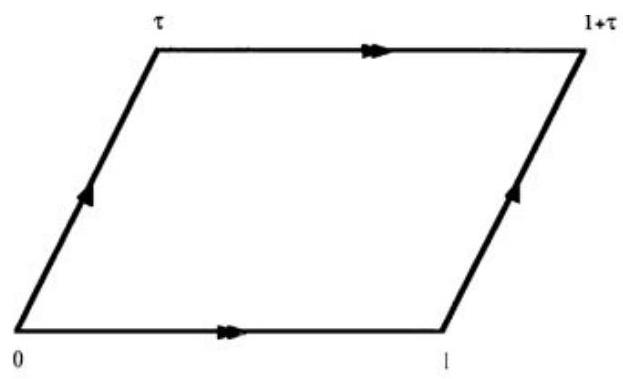
\includegraphics[max width=0.4\textwidth]{images/bo_d3lj80c601uc738kffi0_49_641_372_623_379_0.jpg}
\caption{亏格为 1 的曲线 \(C \cong \mathbb{C} / (\mathbb{Z} \oplus \mathbb{Z}\tau)\)}
\end{figure}

该商空间与平面三次曲线 \(C_3 \subset \mathbb{P}^2_\mathbb{C}\) 之间的同构由一个全纯映射 \(\varphi: \mathbb{C} \to C_3\) 给出，这是 \(C_3\) 的一种“参数化”。但 \(\varphi\) 不能用有理函数表示（见 (2.2)），并且是无限对一的。这就是复变量的双周期函数理论，它是 19 世纪分析学的支柱之一（例如魏尔斯特拉斯 \(\wp\) 函数、黎曼 \(\theta\) 函数）。

另一个重要的注意点是，不同的周期格点 \(\tau\) 通常会导致不同的曲线。它们在拓扑上都同胚于标准环面 \(S^1 \times S^1\)，但作为代数曲线或复解析曲线，它们并不同构。周期 \(\tau\) 是一个模（modulus），即一个复参数，它控制着固定拓扑对象 \(S^1 \times S^1\) 上的复结构 \(C\) 的变化。

对曲线感兴趣的学生应参考 D. Mumford 的《Curves and their Jacobians》，其第一部分较为通俗，或 C. H. Clemens 的《A Scrapbook of Complex Curve Theory》。

\begin{center}
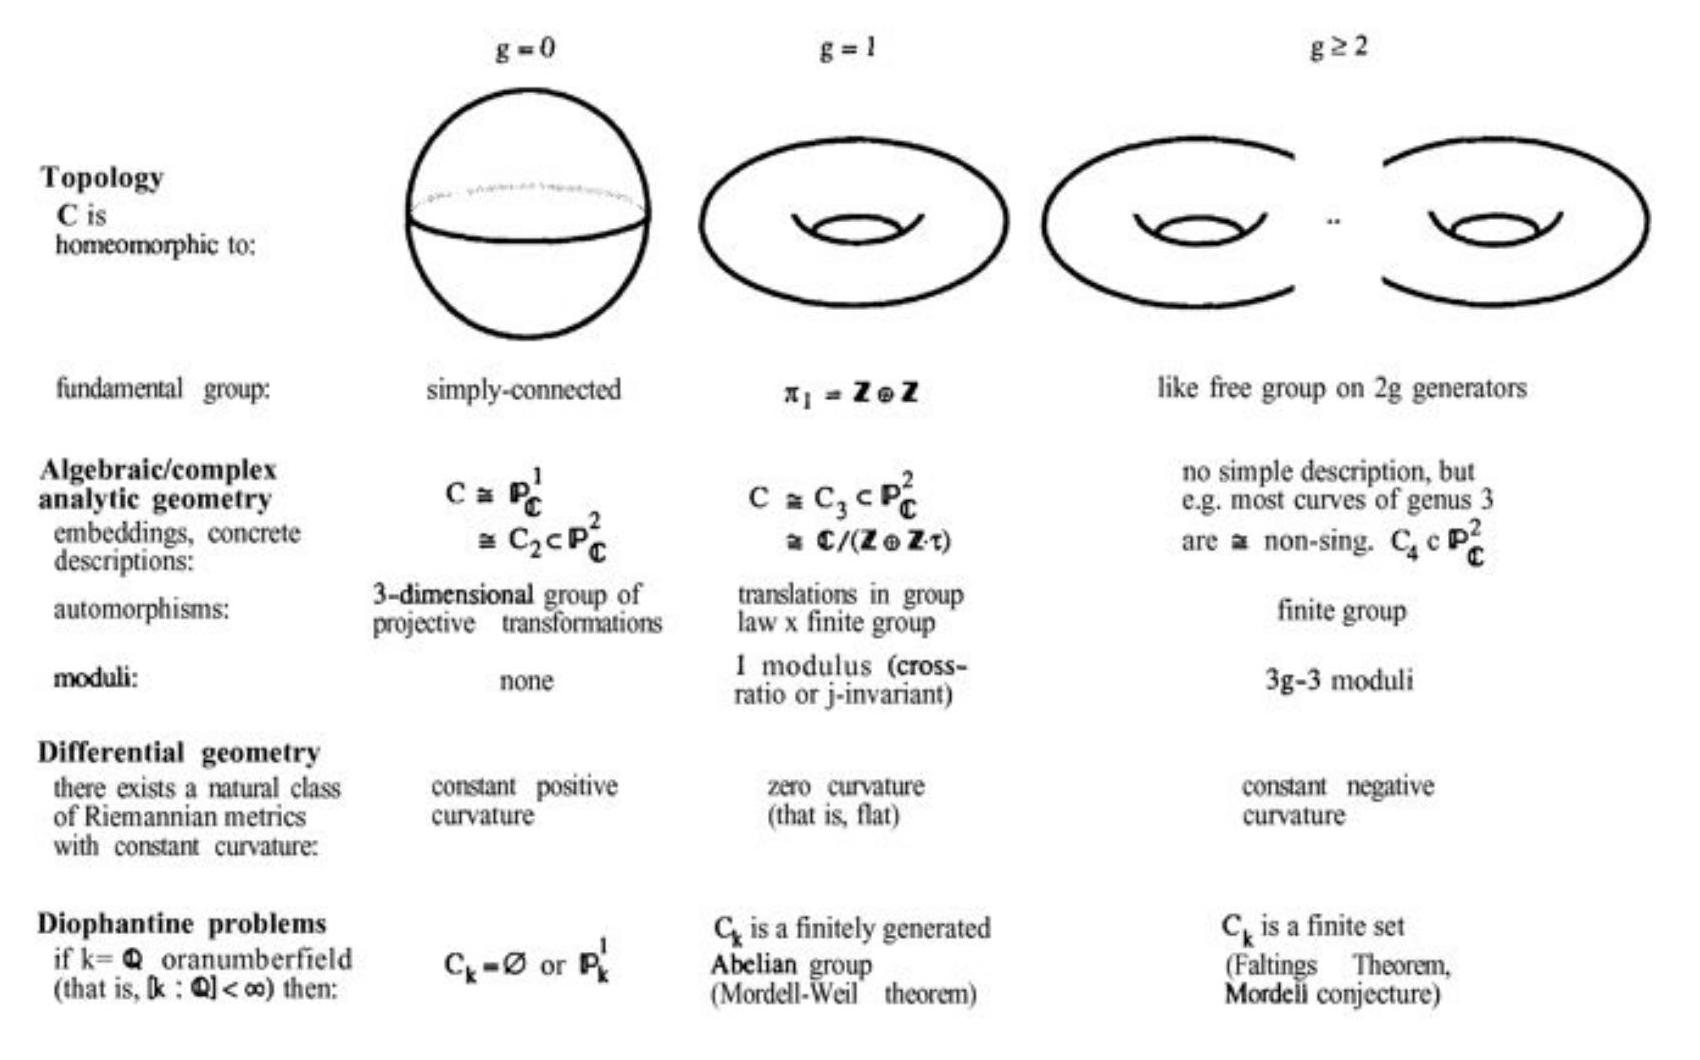
\includegraphics[max width=0.8\textwidth]{images/bo_d3lj80c601uc738kffi0_50_333_253_1060_1700_-1.jpg}
\end{center}
\hspace*{3em}